\documentclass[11pt]{article}
\usepackage[margin=1in]{geometry}
\usepackage{amsmath,amssymb}
\usepackage{graphicx}
\usepackage{microtype}
\usepackage[hidelinks]{hyperref}
\setlength{\emergencystretch}{2em}

\newcommand{\D}{\mathbb D}
\newcommand{\A}{\mathcal A}
\newcommand{\E}{\mathbb E}

\title{\textbf{Contractive Embeddings Between Weighted Bergman Spaces}\\
A Full Literature-Implied Answer to arXiv:1701.06897}
\author{Status note for arXiv:1701.06897}
\date{12 August 2026}

\begin{document}
\maketitle

\begin{center}
\fbox{\parbox{0.91\textwidth}{
\textbf{Status: full literature-implied answer.}
The answer is affirmative for every parameter in the question.  The critical
embedding is Kulikov's 2022 theorem; the extension to the full parameter
wedge is an elementary radial stochastic-order argument.  This note does not
claim an original theorem.
}}
\end{center}

\section{The source question}

For $s>0$ and $\gamma>1$, write
\[
 \|f\|_{A_\gamma^s}^s
 =\int_\D |f(z)|^s(\gamma-1)(1-|z|^2)^{\gamma-2}\,dA(z),
 \qquad dA(z)=\frac{dx\,dy}{\pi},
\]
and use the endpoint convention $A_1^s=H^s$.  The source asks whether
\begin{equation}
 \|f\|_{A_\beta^q}\leq \|f\|_{A_\alpha^p}
 \label{eq:question}
\end{equation}
whenever
\[
 0<p\leq q,\qquad \alpha,\beta\geq1,
 \qquad \frac q\beta\leq\frac p\alpha .
\]
The question begins on PDF p.~9 and continues on p.~10
\cite{BayartEtAl2017}.

\begin{figure}[ht]
\centering

\includegraphics[width=\textwidth]{figures/open_question_crop.png}
\vspace{2mm}
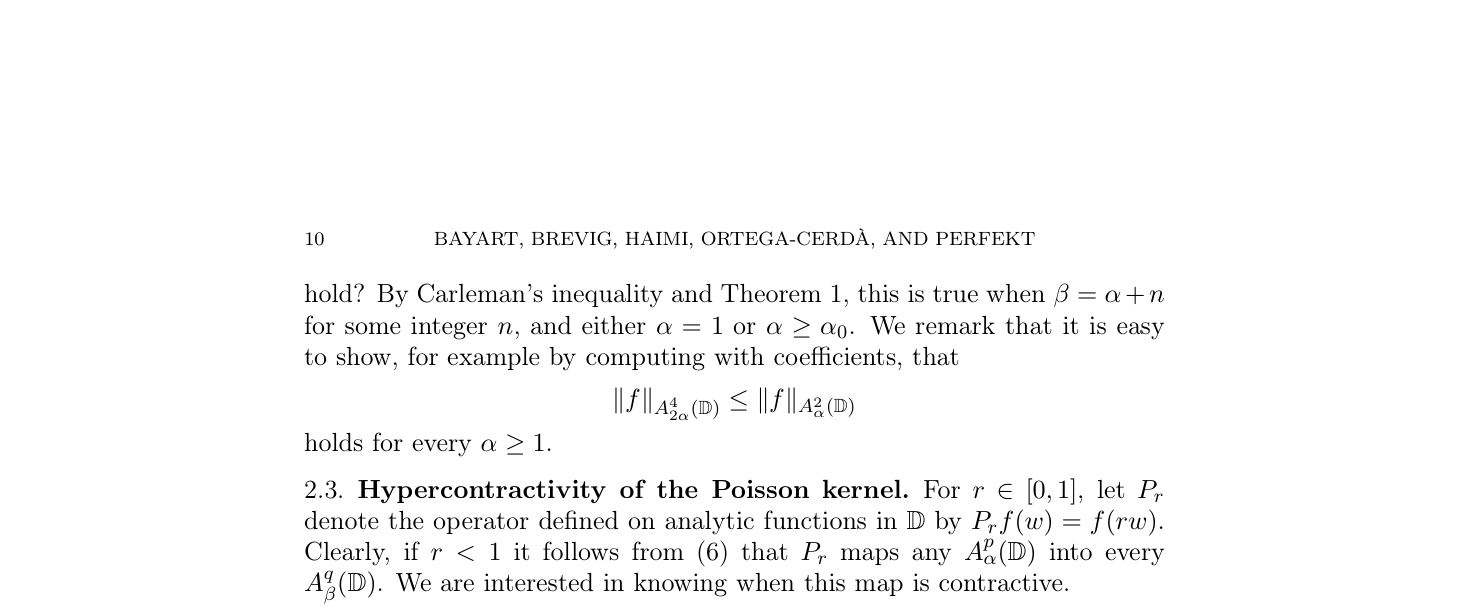
\includegraphics[width=\textwidth]{figures/open_question_continuation_crop.png}
\caption{The question in arXiv:1701.06897, PDF pp.~9--10.}
\end{figure}

\section{Answer}

\paragraph{Theorem.}
Inequality \eqref{eq:question} holds for every analytic $f$ and every set of
parameters appearing in the source question.

\section{Idea / proof intuition}

Set
\[
 \beta_0:=\frac{\alpha q}{p}.
\]
The source hypothesis is exactly $\beta\geq\beta_0$.  Kulikov's theorem gives
the hard step: contractivity at the critical line
$p/\alpha=q/\beta_0$.  It remains only to observe that, for a fixed exponent,
increasing the Bergman weight parameter moves normalized radial mass toward
the origin.  Since the circular integral means of $|f|^q$ increase with the
radius, this can only decrease the norm.  Thus
\[
 A_\alpha^p \hookrightarrow A_{\beta_0}^q
 \hookrightarrow A_\beta^q
\]
contractively.

\section{Proof}

For $s>0$, define the circular integral mean
\[
 M_s(r;f):=\frac1{2\pi}\int_0^{2\pi}
             |f(re^{i\theta})|^s\,d\theta .
\]
Because $|f|^s$ is subharmonic, $M_s(r;f)$ is nondecreasing in $r$.

We first record the promised monotonicity in the weight.  If $\gamma>1$ and
$X_\gamma$ is a random variable on $[0,1]$ with density
\[
 (\gamma-1)(1-x)^{\gamma-2}\,dx,
\]
then polar coordinates give
\begin{equation}
 \|f\|_{A_\gamma^s}^s
 =\E\,M_s(\sqrt{X_\gamma};f).
 \label{eq:expectation}
\end{equation}
Moreover,
\[
 \mathbb P(X_\gamma>t)=(1-t)^{\gamma-1}
 \qquad(0\leq t\leq1).
\]
Consequently, if $\gamma_2\geq\gamma_1>1$, then $X_{\gamma_2}$ is
stochastically smaller than $X_{\gamma_1}$.  Applying this to the increasing
function $x\mapsto M_s(\sqrt{x};f)$ in \eqref{eq:expectation} yields
\begin{equation}
 \|f\|_{A_{\gamma_2}^s}
 \leq \|f\|_{A_{\gamma_1}^s}.
 \label{eq:weightmono}
\end{equation}
If $\gamma_1=1$, the same conclusion follows from
$M_s(r;f)\leq\|f\|_{H^s}^s$; hence \eqref{eq:weightmono} is valid with the
Hardy endpoint as well.

Suppose first that $p<q$.  If $\alpha>1$, Kulikov's Corollary~1.3 applies to
$p,q,\alpha,\beta_0$, since
\[
 \frac p\alpha=\frac q{\beta_0},
\]
and gives
\begin{equation}
 \|f\|_{A_{\beta_0}^q}
 \leq \|f\|_{A_\alpha^p}.
 \label{eq:critical}
\end{equation}
The same corollary contains the Hardy endpoint when $\alpha=1$: indeed its
rightmost inequality is
$\|f\|_{A_{q/p}^q}\leq\|f\|_{H^p}$.

\begin{figure}[ht]
\centering
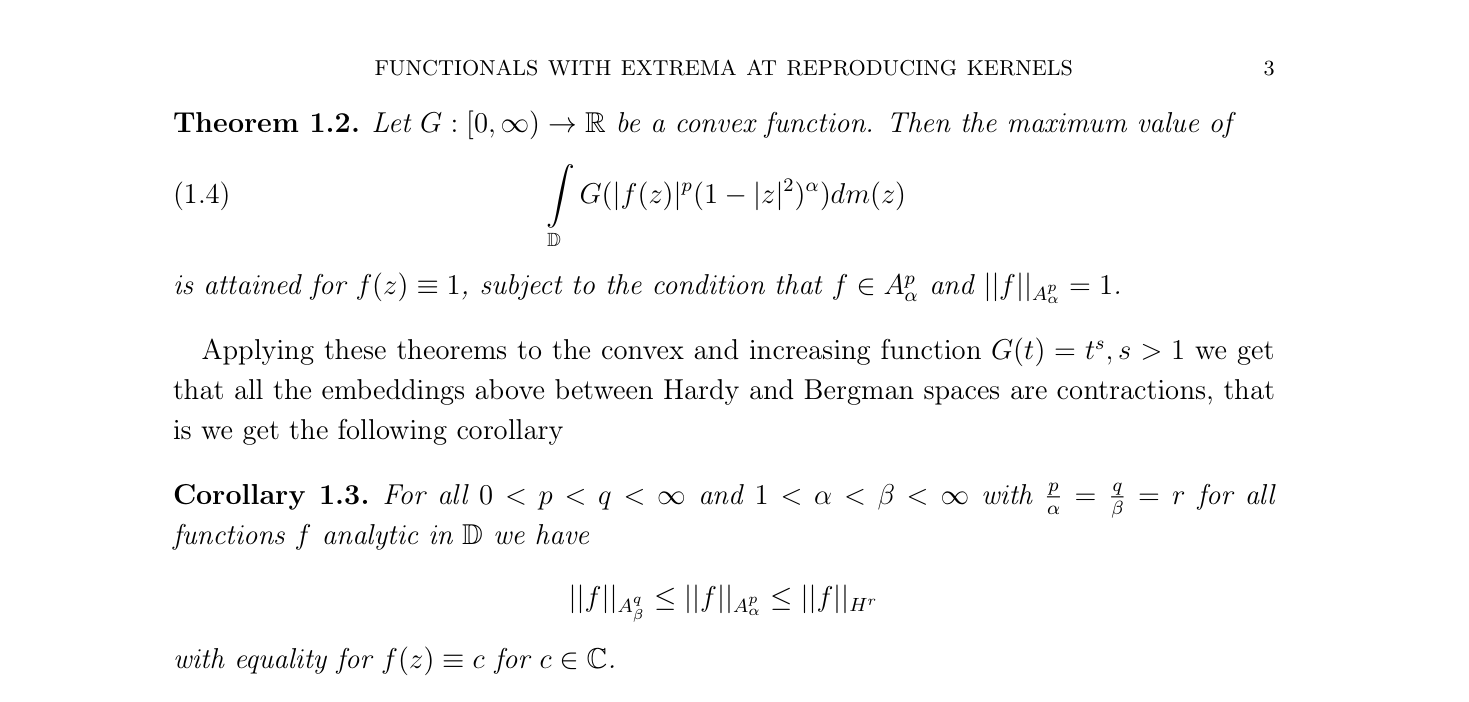
\includegraphics[width=\textwidth]{figures/supporting_corollary_crop.png}
\caption{Kulikov's critical-line contraction and Hardy endpoint
\cite[Corollary 1.3]{Kulikov2022}.}
\end{figure}

Since the source hypothesis says $\beta\geq\beta_0$, combining
\eqref{eq:weightmono} with \eqref{eq:critical} gives
\[
 \|f\|_{A_\beta^q}
 \leq \|f\|_{A_{\beta_0}^q}
 \leq \|f\|_{A_\alpha^p},
\]
which is \eqref{eq:question}.

Finally, if $p=q$, the hypothesis is simply $\beta\geq\alpha$, so
\eqref{eq:question} follows directly from \eqref{eq:weightmono}; the case
$\alpha=\beta=1$ is equality.  This exhausts all endpoints and completes the
proof. \hfill$\square$

\section{Provenance and scope}

Kulikov's paper appeared after the 2017 source and explicitly proves that the
critical Hardy--Bergman and Bergman--Bergman embeddings are contractions.
The passage from the critical line to all $\beta\geq\beta_0$ is the elementary
monotonicity argument \eqref{eq:weightmono}.  The exact source question is
therefore fully resolved, but the result is classified as
\emph{literature-implied}, not as an original result of this run.

This note answers only the displayed one-variable weighted Bergman embedding
question.  It makes no claim about the source's separate infinite-polydisk
Carleson-measure question or its multiplicative-Hankel-form questions.

\begin{thebibliography}{9}

\bibitem{BayartEtAl2017}
F.~Bayart, O.~F.~Brevig, A.~Haimi, J.~Ortega-Cerd\`a, and K.-M.~Perfekt,
\emph{Contractive inequalities for Bergman spaces and multiplicative Hankel
forms}, arXiv:1701.06897v2, 2017.

\bibitem{Kulikov2022}
A.~Kulikov,
\emph{Functionals with extrema at reproducing kernels},
Geom. Funct. Anal. \textbf{32} (2022), 938--949;
\href{https://arxiv.org/abs/2203.12349}{arXiv:2203.12349}.

\end{thebibliography}

\end{document}
